\chapter{Security}

\section{Cryptographic Techniques}
\subsection{Problems and Goals}
\begin{itemize}
    \item Authentication: who am I talking to?
    \item Confidentiality: is my data hidden?
    \item Integrity: is my data changed?
\end{itemize}

\subsection{Kinds of Cryptography}
\begin{table}
\centering
\caption{Compare between two Cryptography}
\label{tab:1}
\begin{tabular}{lll}
\hline\noalign{\smallskip}
 & Symmetric & Asymmetric  \\
\noalign{\smallskip}\hline\noalign{\smallskip}
Shared Secret & Yes & No \\
Speed & Fast & Slow \\
\noalign{\smallskip}\hline
\end{tabular}
\end{table}

\subsubsection{Symmetric Cryptography}
\textbf{Confidentiality: One-time Pad (OTP)}
\begin{itemize}
    \item Key is as long as the message.
    \item One-time key.
    \item Two kinds: stream cipher and block cipher.
\end{itemize}

\textbf{Integrity: Hash Message Authentication Code (HMAC)}
\paragraph{Hashing for Cryptography}
Properties:
\begin{itemize}
    \item Consistent: same input, same output.
    \item One-way: have $Y$, cannot get $X$.
    \item Collision resistant: different input, different output.
\end{itemize}

\begin{enumerate}
    \item Sender creates a hashed message (MAC) and attach it with the content message;
    \item Receiver computes the MAC with message and verify the integrity of the message.
\end{enumerate}

\textbf{Authentication: HMAC and Nonce}

Much similar with the verification in integrity.


\subsubsection{Asymmetric Cryptography}
Instead of shared keys, each person has a key pair: public key and private key.

The public key of a holder will be used by others, and private key will be used by itself.

The authentication will be against the holder of a key, so that the message should be first signed by the private key of the holder. Then the receiver can verify it with public key.

\section{Key Distribution and Management}
\subsubsection{Why use a central key server?}
Each pair of hosts have a pair of keys $-> n^2$ keys

\subsection{Key Distribution Center (KDC) - Kerberos}
\subsubsection{What is the setting?}
\begin{itemize}
    \item Alice and Bob know own symmetric keys for KDC (KDC holds different symmetric keys with each registered user).
    \item Alice and Bob ask the KDC to get a symmetric key for communication.
\end{itemize}

\subsubsection{How two hosts communicate with KDC?}
\begin{enumerate}
    \item By using $K_{A-KDC}$, Alice asks KDC to generate a symmetric key for communication with Bob.
    \item KDC generates $R_1$ for the communication, and send $(R1, K_{B-KDC})$ to Alice
    \item Alice use $(R1, K_{B-KDC})$ to communicate with Bob.
    \item Bob knows using $R_1$ as the session key to communicate with Alice.
\end{enumerate}

\subsubsection{Why use KDC?}
\begin{itemize}
    \item Centralized trust and failure.
    \item KDC can expose session keys to others
\end{itemize}

\subsubsection{Kerberos: authentication before using service}
The client authenticates itself to the Authentication Server (AS) which forwards the username to a key distribution center (KDC). The KDC issues a ticket-granting ticket (TGT), which is time stamped, encrypts it using the user's password and returns the encrypted result to the user's workstation. This is done infrequently, typically at user logon; the TGT expires at some point, though may be transparently renewed by the user's session manager while they are logged in.

When the client needs to communicate with another node ("principal" in Kerberos parlance) the client sends the TGT to the ticket-granting service (TGS), which usually shares the same host as the KDC. After verifying the TGT is valid and the user is permitted to access the requested service, the TGS issues a ticket and session keys, which are returned to the client. The client then sends the ticket to the service server (SS) along with its service request.

\begin{figure}
\centering
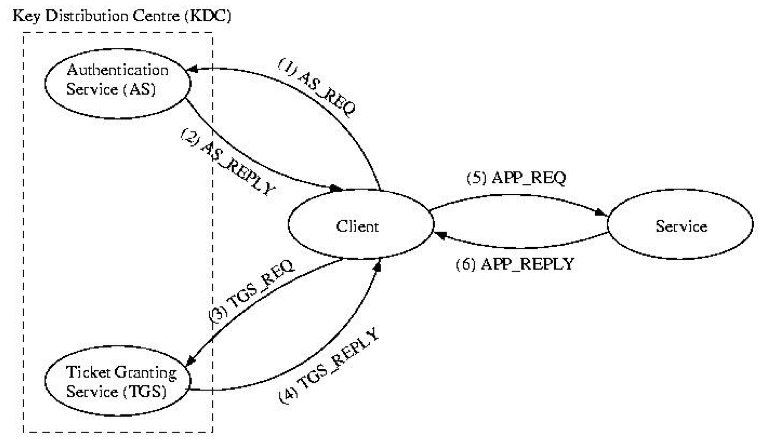
\includegraphics[width=\textwidth]{img/ch06-kerberos.png}
\caption{Kerberos}
\label{fig:ch06-kerberos}
\end{figure}

How the procedure works:
\begin{enumerate}
    \item Client asks AS for authentication: AS issues a TGT and session key to the client. TGT cannot be read by client, it is for TGS. Session key is used for later encryption. 
    \item Client uses the TGT to ask TGS for a service ticket. At the same time, use session key to communicate with TGS. The service ticket also cannot be read by client.
    \item Client uses the service ticket to request service servers. At the same time, use session key to communicate with service server.
\end{enumerate}